\PassOptionsToPackage{colorlinks=true,citecolor=blue, linkcolor=metropolis_border_color}{hyperref} % override theme hyperref to set a citation color. 
\documentclass[11pt]{beamer}
\usetheme{metropolis}
\usepackage[utf8]{inputenc}

\usefonttheme{professionalfonts} % using non standard fonts for beamer
\usefonttheme{serif} % default family is serif
\usepackage{fontspec}
\setmainfont{Satoshi}

%\usepackage{natbib}
%  \setcitestyle{square,numbers,sort&compress}
%  \setcitestyle{sort&compress}

\usepackage[style=numeric, maxbibnames=3, minbibnames=3, sorting=none, backend=bibtex]{biblatex}
%\usepackage[style=numeric, maxbibnames=3, minbibnames=3, backend=biber]{biblatex}
\addbibresource{references.bib}
\usepackage{hypernat} % hypernat also required to allow citations to compress. 

\usepackage{amsmath}
\usepackage{amsfonts}
\usepackage{amssymb}
\usepackage{graphicx}
\graphicspath{ {images/} } % sets the path to image files (Figures)
\usepackage[export]{adjustbox}
\setlength{\fboxsep}{0pt} % Adjust the padding inside the box
\setlength{\fboxrule}{1pt} % Adjust the thickness of the border
\usepackage{xcolor}
\definecolor{metropolis_border_color}{RGB}{35, 55, 59}

\usepackage{calc} % for cropped image calc
\newlength{\imagewidth}
\newlength{\imageheight}
\usepackage{tikz}

\author{Dylan Lawless}
\title{

\includegraphics[height=.12\textheight,valign=c]{SwissPedHealth_Pipeline_Devs.png}
\hspace{0em}
SwissPedHealth Analysis pipelines
}
%\setbeamercovered{transparent} 
%\setbeamertemplate{navigation symbols}{} 
%\logo{} 
%\institute{} 
\date{July 02, 2023} 
%\subject{} 
\begin{document}

%%%%%%%%%% %%%%%%%%%% %%%%%%%%%%
\begin{frame}
\titlepage
\end{frame}

\begin{frame}{Content}
\tableofcontents
\end{frame}


%%%%%%%%%% %%%%%%%%%% %%%%%%%%%%
\section{Bioinformatics}

\begin{frame}{Bioinformatics}
  \begin{columns}
    \column{.4\textwidth}
    \fcolorbox{metropolis_border_color}{white}{
\includegraphics[height=.8\textheight]{SwissPedHealth_Pipeline_Devs.png}}
    
    \column{.6\textwidth}
      \hfill % Add horizontal space between the columns
    \fcolorbox{metropolis_border_color}{white}{
\includegraphics[height=.36\textheight]{SwissPedHealth_Pipeline_Devs.png}}
    
    % \vspace{1em} % Adjust the vertical spacing between the two graphics
    \hfill % Add horizontal space between the columns
    \fcolorbox{metropolis_border_color}{white}{
\includegraphics[height=.36\textheight]{SwissPedHealth_Pipeline_Devs.png}}
  \end{columns}
\end{frame}

%%%%%%%%%% %%%%%%%%%% %%%%%%%%%%
\begin{frame}[standout]
\vspace{4em}
\begin{center}

\includegraphics[height=.12\textheight,valign=c]{SwissPedHealth_Pipeline_Devs.png}
\hspace{0em}
SwissPedHealth Analysis pipelines
\end{center}    
\vspace{4em}
\makebox[\linewidth]{\vspace{20em}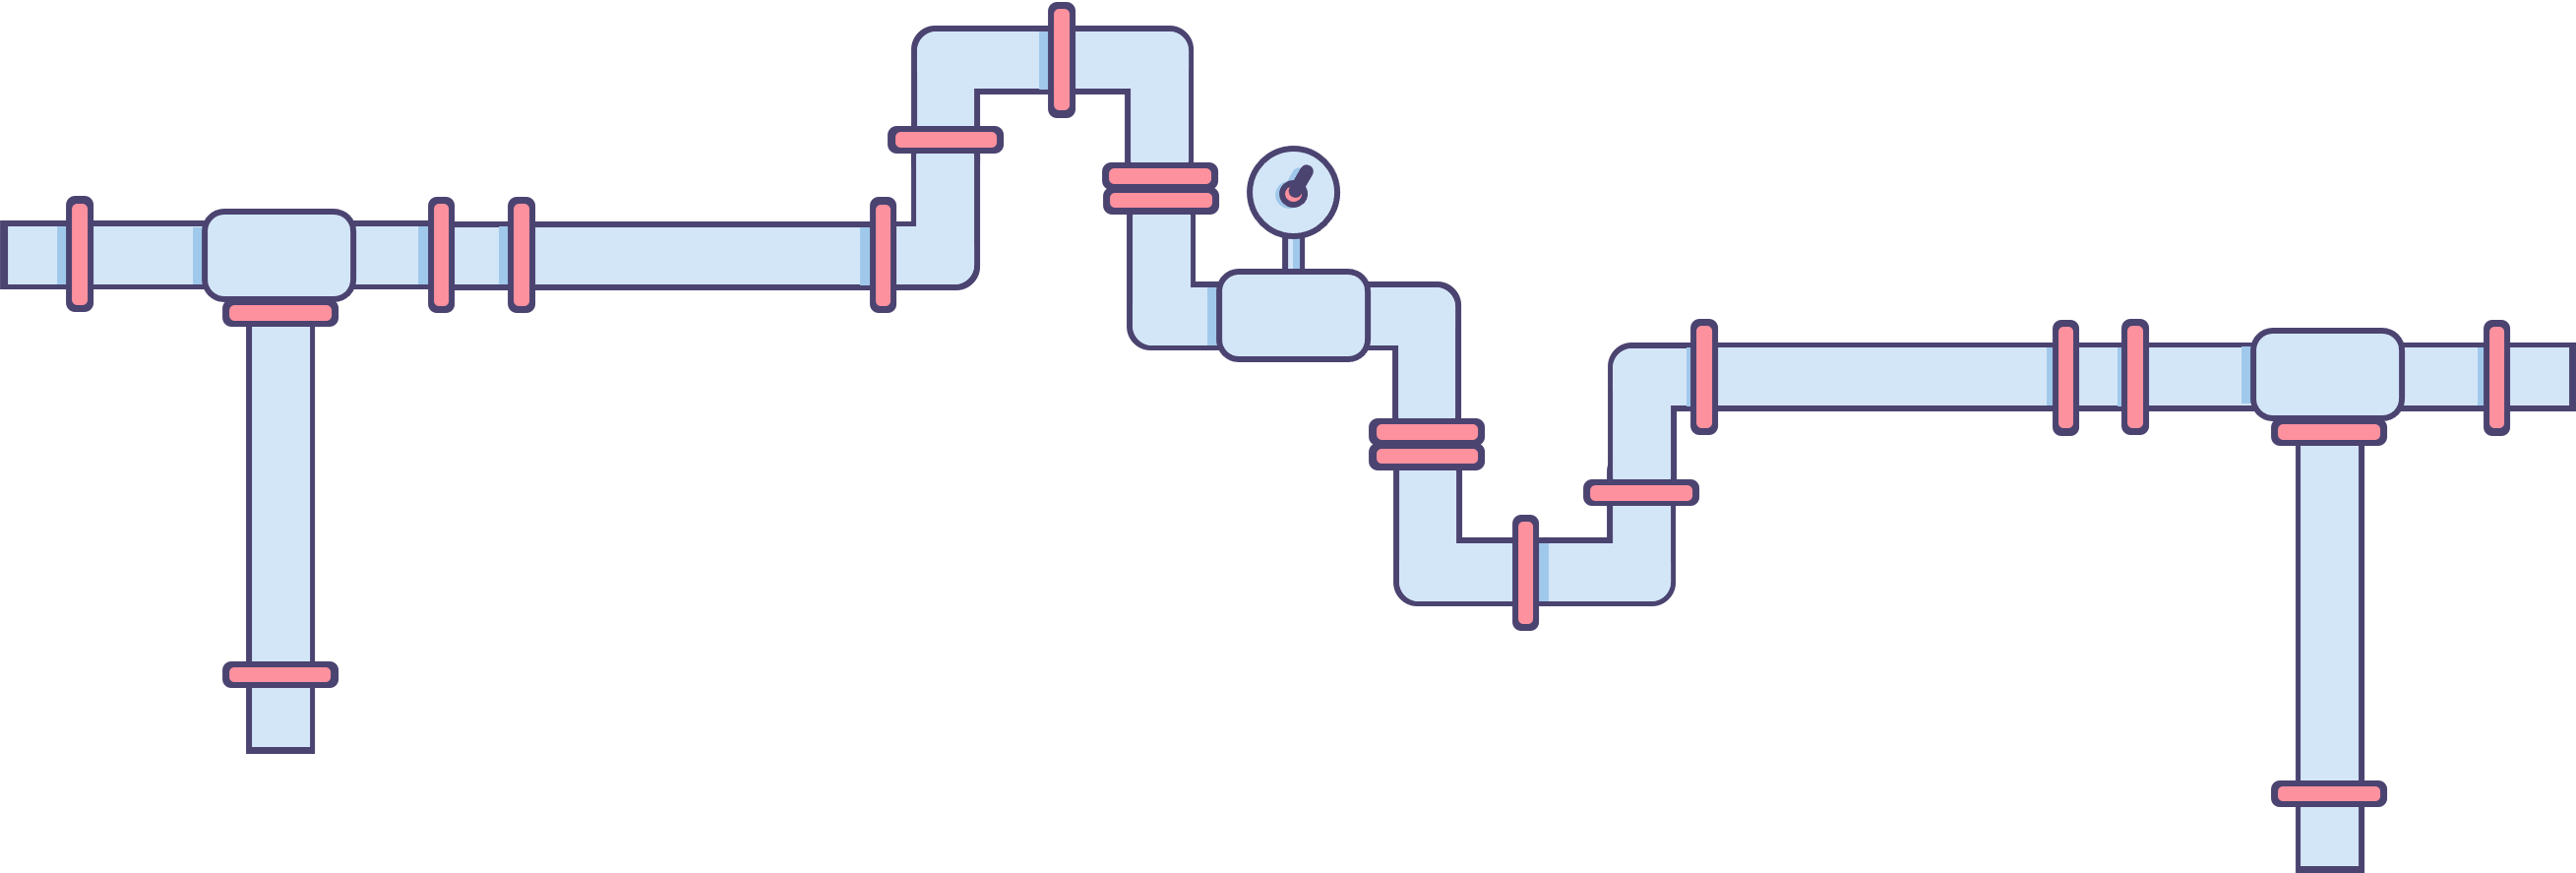
\includegraphics[width=1.2\linewidth, valign=b]{SwissPedHealth_Pipeline_Devs_wide_2.png}}

\cite{Povysil2019rare}
\end{frame}

%%%%%%%%%% %%%%%%%%%% %%%%%%%%%%
\begin{frame}[allowframebreaks]
       \frametitle{References}
        \renewcommand*{\bibfont}{\tiny}
%\bibliographystyle{unsrtnat}
%\bibliography{references}
\printbibliography[heading=none]

   
\end{frame}

\begin{frame}{notes}
BiomedIT

Aidan Ruppel (?), who sits with Julia Ruppel and Tatiana, on call might be good to ask about training and documentation. 

Data agreements - 
op1 - SwissPedHealth legal
op2 - SPO style legal

They prefer op2. 

SMOC people to talk to: Patrick Pedrioli, Katrin Mannik.  

\end{frame}

\end{document}